\documentclass{article}
\usepackage[utf8]{inputenc}
\usepackage[letterpaper,margin=1in]{geometry}
\usepackage{graphicx}
\usepackage{listings}
\usepackage{color}
\usepackage{hyperref}
\usepackage{multirow}

\definecolor{mine}{rgb}{0,0,0.7}
\hypersetup{
    colorlinks=true,
    linkcolor=mine,
    citecolor=mine,
    urlcolor=mine,
    pdftitle={SPOTs Imager},
}

\definecolor{dkgreen}{rgb}{0,0.6,0}
\definecolor{gray}{rgb}{0.5,0.5,0.5}
\definecolor{mauve}{rgb}{0.58,0,0.82}

\lstset{frame=tb,
  language=matlab,
  aboveskip=3mm,
  belowskip=3mm,
  showstringspaces=false,
  columns=flexible,
  basicstyle={\small\ttfamily},
  numbers=none,
  numberstyle=\tiny\color{gray},
  keywordstyle=\color{blue},
  commentstyle=\color{dkgreen},
  stringstyle=\color{mauve},
  breaklines=true,
  breakatwhitespace=true,
  tabsize=3
}

\title{Scanning Imager Guide}
\author{Mark Menesses}
\date{15 September 2020}

\begin{document}

\maketitle

\tableofcontents
\newpage

\section{Overview}
The SPOTs scanning imager allows for programmatic imaging of SPOTs across a large area (30cm x 30cm).
\section{Hardware}
The system is comprised of a motorized X-Y stage and an imaging head.
The system is controlled using Gcode fed into a GRBL controller.
\subsection{Stage}
The current stage in use is the \href{https://openbuilds.com/builds/openbuilds-acro-system.5416/}{ACRO 55} purchased from \href{https://openbuilds.com/}{OpenBuilds}.
This stage offers X and Y movement over a 12''x12'' area.
Some specs:

\begin{tabular}{l l}
     Drive System: & Belt Driven GT2 timing belts \\
     Machine Accuracy: & 0.003"~0.007" (0.10mm~0.20mm) (This seems off. Might be more like $\pm$0.05mm) \\
     Footprint: & 20" x 20" (500mm x 500mm) \\
     Motors: & NEMA 17 \\
     Controller: & OpenBuilds BlackBox \\
\end{tabular}


\begin{figure}[!h]
    \centering
    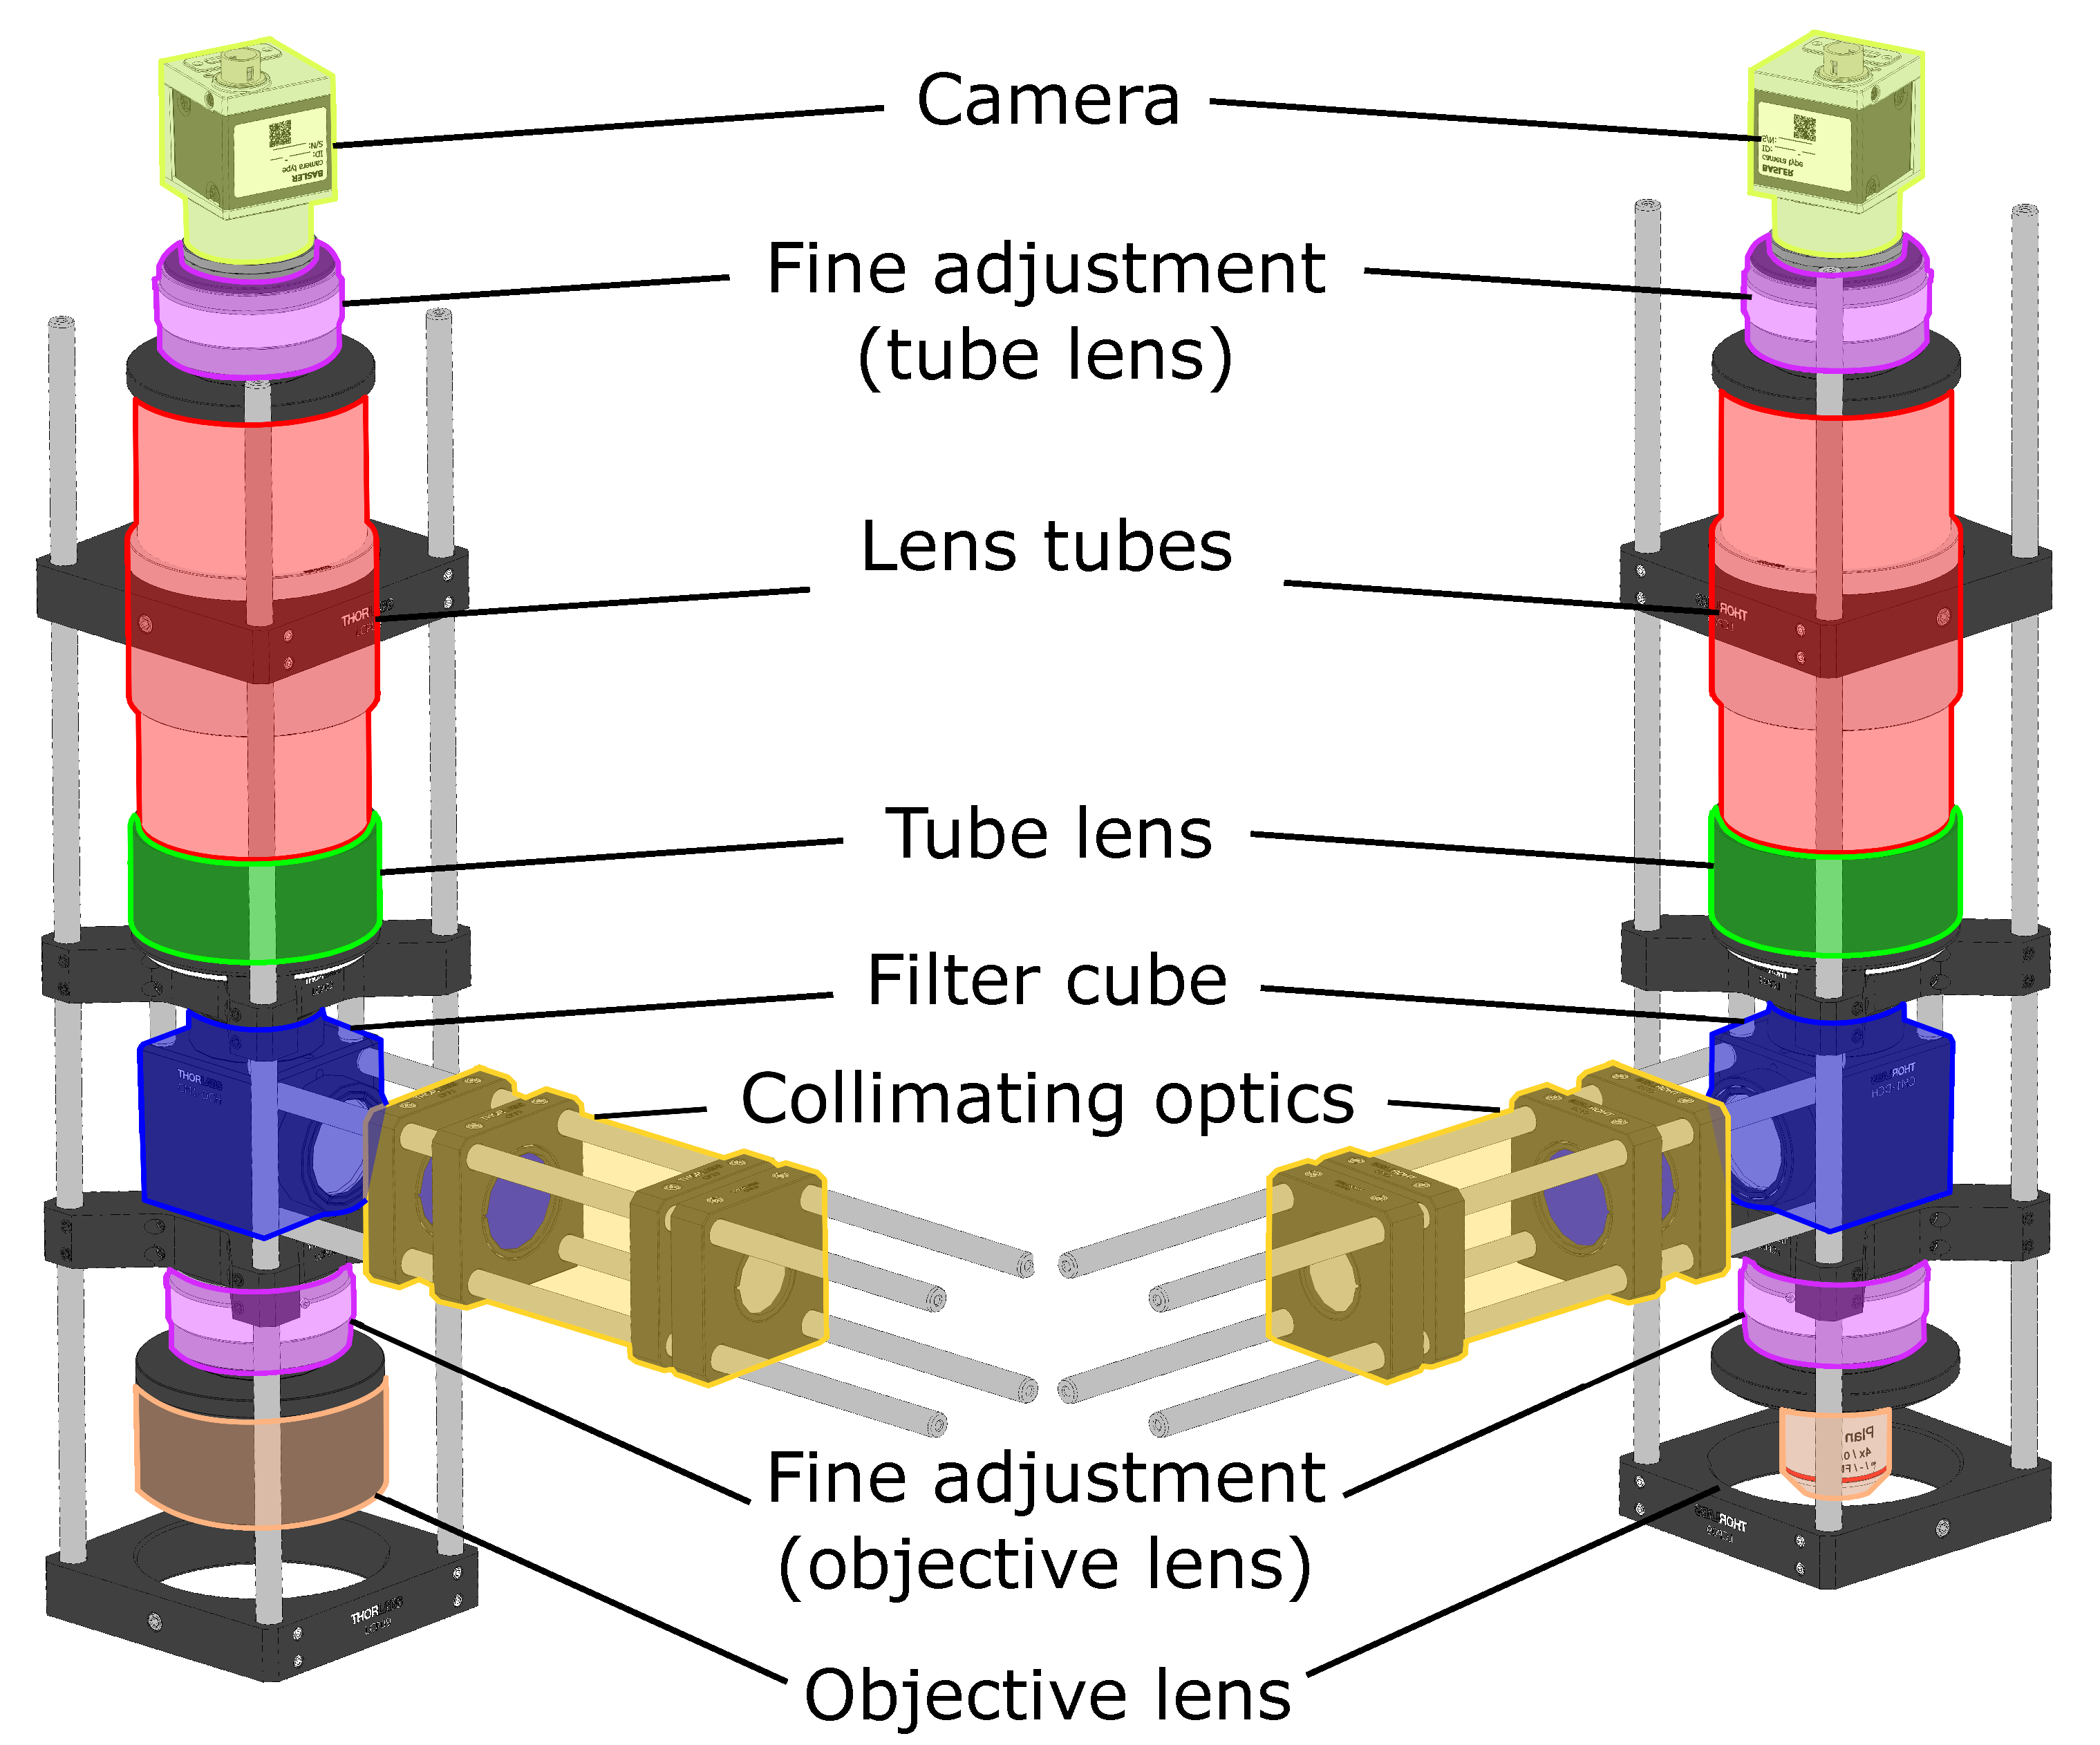
\includegraphics[width=0.75\columnwidth]{imager_sketch.eps}
    \caption{Sketch of imaging components. The left configuration shows an achromatic lens used as the objective, while the right shows an infinity corrected microscope objective in use.}
    \label{fig:sketch}
\end{figure}

\subsection{Camera}
	
A variety of cameras may be used with a preference for smaller, C-mount cameras for weight purposes.
The camera should be supported by MATLAB's Image Acquisition toolbox for ease of integration.
Currently, we use a \href{https://www.baslerweb.com/en/products/cameras/area-scan-cameras/ace/aca3800-14uc/}{Basler acA3800-14uc} (specs below).

\begin{tabular}{l l}
    Sensor Size: & 6.4mm x 4.6 mm \\
    Resolution: & 3840 px x 2748 px (10 MP) \\
    Pixel Size: & 1.67 $\mu$m x 1.67 $\mu$m \\
    Max. Frame Rate (at full res.): & 14 fps \\
    Pixel Bit Depth: & 12 bits
\end{tabular}

\subsection{Optics}
A custom set of optics is being used to achieve a range of magnifications and enable the use of epifluorescence.
Optical components for the collimation of the excitation light were duplicated from the Thorlabs WFA2001 module.
Two lenses are used in the system, an objective lens and a tube lens, between which sets up an infinity space between them in which we introduce our epi-illumination.
The available lenses are listed in Table \ref{tab:lenses}.
The range of magnifications available for a given lens pair is listed in Table \ref{tab:magnifications}.

\begin{table}[!h]
\centering
\begin{tabular}{c c c c c c}
    \textbf{Lens}  & \textbf{Description} & \textbf{Thorlabs PN} & \textbf{Focal Length} & \textbf{Working Distance} & \textbf{Magnification} \\
    A & Achromatic lens & AC508-100-A & 100 mm & 89.0 mm & --- \\
	B & Achromatic lens & AC508-150-A & 150 mm & 140.4 mm & --- \\
	C & Achromatic lens & AC508-180-A & 180 mm & 172.7 mm & --- \\
	D & Achromatic lens & AC508-200-A & 200 mm & 193.7 mm & --- \\
	E & Plan N 4x & RMS4X & 180 mm & 18.5 mm & 4x 
\end{tabular}
\caption{Lens choices and properties}
\label{tab:lenses}
\end{table}

\bgroup
\def\arraystretch{1.35}
\begin{table}[!h]
    \centering
    \begin{tabular}{c c|c|c|c|c}
           & & \multicolumn{4}{c}{\textbf{Tube Lens}} \\
           & &  A   &  B   &  C   &  D  \\
           \hline
        \multirow{5}{*}{\rotatebox[origin=c]{90}{\textbf{Objective Lens}}} & A & ---  & 1.50 & 1.80 & 2.00 \\ \cline{2-6}
         & B & 0.67 & --- & 1.20 & 1.33 \\ \cline{2-6}
         & C & 0.56 & 0.83 & --- & 1.11 \\ \cline{2-6}
         & D & 0.50 & 0.75 & 0.90 & --- \\ \cline{2-6}
         & E & 2.22 & 3.33 & 4.00 & 4.444 \\
    \end{tabular}
    \caption{Magnifications achieved by varying lens combinations}
    \label{tab:magnifications}
\end{table}
\egroup

\section{Setup}
\subsection{Select magnification}
Use Table \ref{tab:magnifications} to select the appropriate lenses for the desired magnification.
\subsection{Install lenses}
Lenses installed on the system as shown in Figure \ref{fig:sketch}.
Each achromatic lens is mounted within its own threaded housing.
To install these lenses in the objective position, they should be screwed into the thread adapter below the fine focus adjustment at the bottom of the assembly (the exterior threads will be facing upwards).

\subsection{Focus optics}
\subsection{}
Prior to operation, the user should select the lenses (Table \ref{tab:lenses}) which will give the appropriate magnification, as given in Table \ref{tab:magnifications}.
The camera must be placed at the working distance of the tube lens.
Currently, a series of threaded lens tubes provides coarse adjustment of this distance, while fine adjustment

\section{Image acquisition workflow}

\section{In progress}
\subsection{Epifluorescence}
We have optics setup that should allow for epifluorescence, but this remains to be tested.
One item to be considered still is the light source.
We can either choose a specific wavelength for a given application, or use a broadband source and filter.
The modular nature of our system requires a rather lightweight source, such as a small LED. One issue may be heating of the light source.
We could consider using the controller PWM pin to turn our light on and off between images.
\subsection{Image stitching}
We have not yet chosen a software for image stitching.
As this is a post-processing step, many options are available.




\section{Cost}
\begin{table}[!h]
\centering
\begin{tabular}{cccccc}
\textbf{Vendor} & \textbf{Part Number} & \textbf{Brief Description}              & \textbf{Qty} & \textbf{Unit Price} & \textbf{Subtotal} \\
 & & & & \textbf{(USD)} & \textbf{(USD)} \\
Thorlabs        & AC508-100-A          & Achromatic Lens, f=100mm                & 1            & 113                       & 113                     \\
Thorlabs        & AC508-150-A          & Achromatic Lens, f=150mm                & 1            & 113                       & 113                     \\
Thorlabs        & AC508-180-A          & Achromatic Lens, f=150mm                & 1            & 113                       & 113                     \\
Thorlabs        & AC508-200-A          & Achromatic Lens, f=100mm                & 1            & 113                       & 113                     \\
Thorlabs        & AL2018-A             & Collimating optics                      & 1            & 240                       & 240                     \\
Thorlabs        & CM1-DCH              & Filter cube                             & 1            & 175                       & 175                     \\
Thorlabs        & CP33                 & Lens housing                            & 3            & 17                        & 51                      \\
Thorlabs        & CPN20                & Lens housing                            & 1            & 34                        & 34                      \\
Thorlabs        & ER1                  & Cage rails                              & 4            & 5                         & 20                      \\
Thorlabs        & ER05                 & Cage rails                              & 4            & 5                         & 20                      \\
Thorlabs        & ER8                  & Cage rails                              & 4            & 12                        & 48                      \\
Thorlabs        & ER12                 & Cage rails                              & 4            & 17                        & 68                      \\
Thorlabs        & LBF254-040-A         & Collimating optics                      & 2            & 57                        & 114                     \\
Thorlabs        & LBF254-100-A         & Collimating optics                      & 1            & 57                        & 57                      \\
Thorlabs        & LCP02                & Cage plate                              & 2            & 42                        & 84                      \\
Thorlabs        & LCP09                & Cage plate                              & 2            & 46                        & 92                      \\
Thorlabs        & MD480                & Dichroic                                & 1            & 237                       & 237                     \\
Thorlabs        & MF434-17             & Excitation Filter                       & 1            & 258                       & 258                     \\
Thorlabs        & MF630-69             & Emission Filter                         & 1            & 258                       & 258                     \\
Thorlabs        & RMS4X                & 4x microscope objective                 & 1            & 146                       & 146                     \\
Thorlabs        & SM1A2                & Thread adapter                          & 3            & 27                        & 81                      \\
Thorlabs        & SM1A9                & Thread adapter                          & 1            & 20                        & 20                      \\
Thorlabs        & SM1L03               & Filter mount/lens tube                  & 4            & 13                        & 52                      \\
Thorlabs        & SM1ZM                & Fine adjustment for optics              & 2            & 176                       & 352                     \\
Thorlabs        & SM2A32               & Thread adapter                          & 1            & 28                        & 28                      \\
Thorlabs        & SM2L10               & Lens housing                            & 4            & 31                        & 124                     \\
Thorlabs        & LCP01B               & Mounting hardware                       & 2            & 32                        & 64                      \\
Thorlabs        & SM2T20               & Lens tube                               & 2            & 41                        & 82                      \\
Thorlabs        & SM2T10               & Lens tube                               & 1            & 39                        & 39                      \\
Thorlabs        & SM2T2                & Lens tube                               & 1            & 38                        & 38                      \\
Thorlabs        & SM2M10               & Lens tube                               & 1            & 30                        & 30                      \\
Thorlabs        & SM2M15               & Lens tube                               & 1            & 31                        & 31                      \\
Thorlabs        & SM2M20               & Lens tube                               & 1            & 33                        & 33                      \\
Edmund Optics   & 89-992               & C-Mount USB Camera                      & 1            & 695                       & 695                     \\
OpenBuilds      & 2365-Bundle          & Stage frame components & 1            & 290                       & 290                     \\
OpenBuilds      & 2790-Kit             & Stage controller                        & 1            & 190                       & 190                     \\
OpenBuilds      & 623                  & Stage motors                            & 3            & 18                        & 54                      \\
OpenBuilds      & 591-Set              & 24V power supply                        & 1            & 70                        & 70                      \\
                &                      &                                         &              &                           & \textbf{4627}          
\end{tabular}
\caption{Bill of materials}
\end{table}

\begin{figure}[!h]
    \centering
    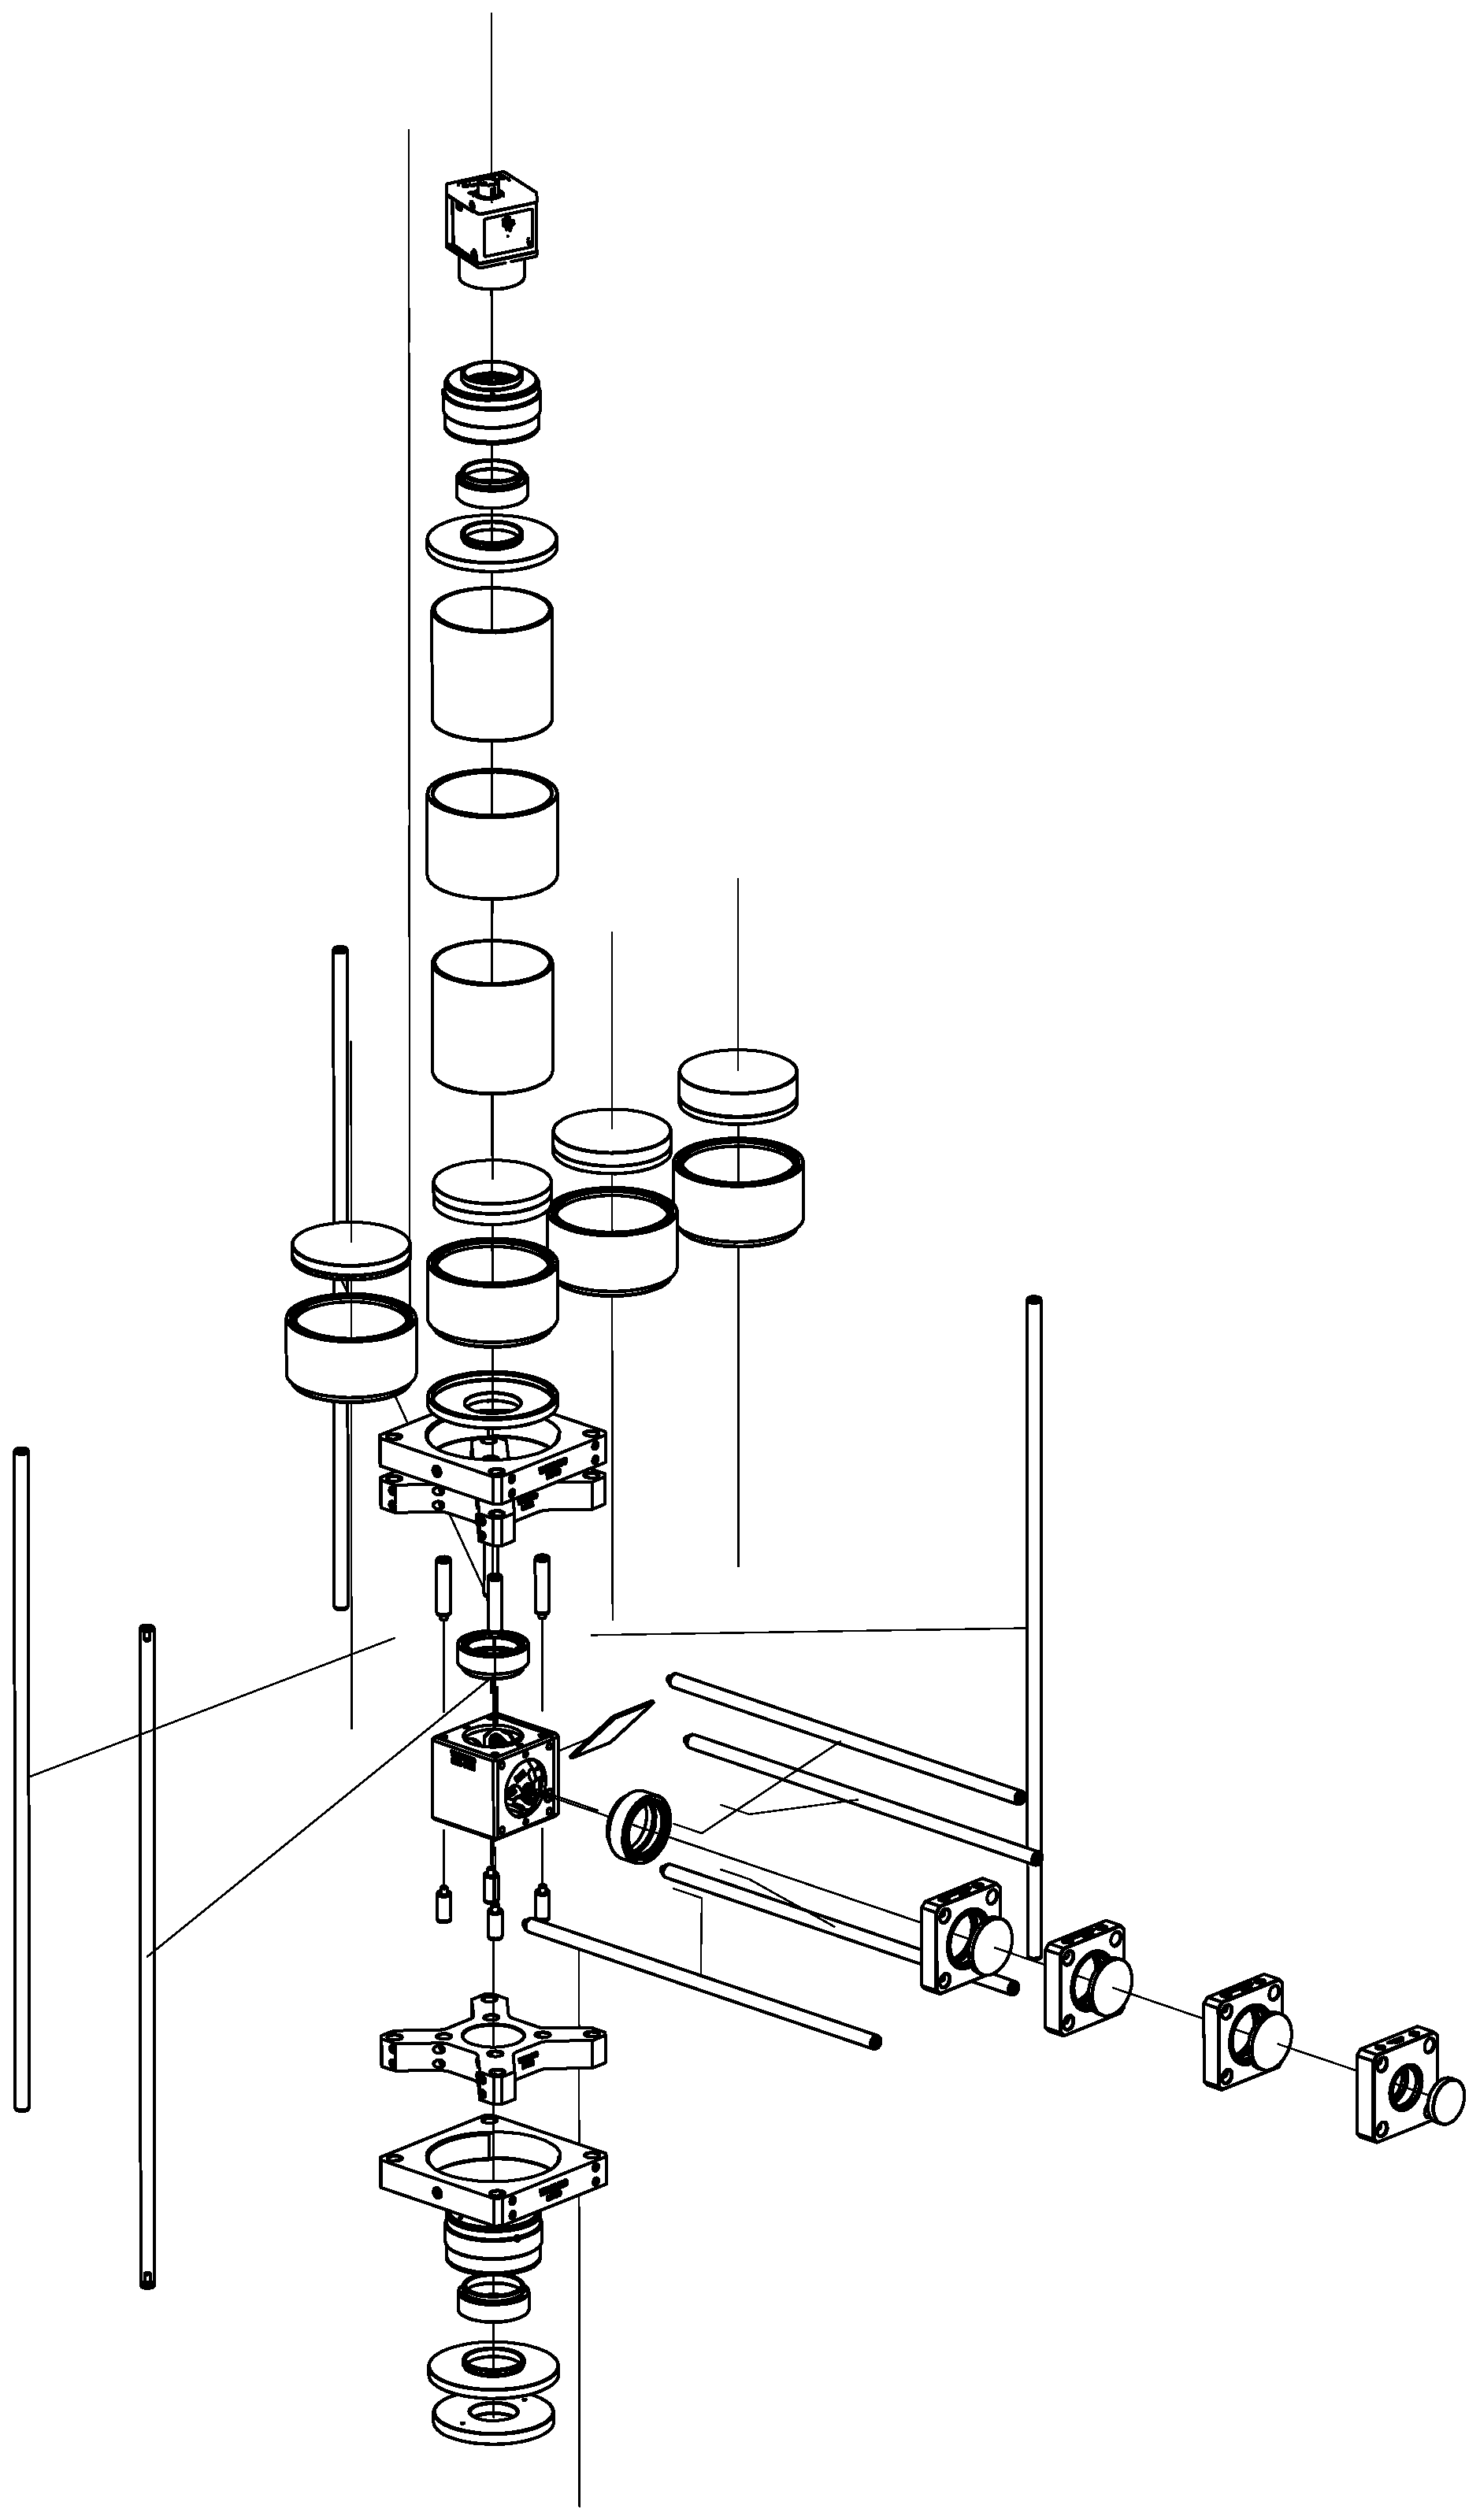
\includegraphics[width = 0.5\columnwidth]{optics_assembly_illustrated_exploded.eps}
    \caption{Exploded schematic of optical assembly}
    \label{fig:my_label}
\end{figure}


\section{MATLAB Code:}
    \subsection{Main Script}
        \input{matlab_files/MAIN}
    \subsection{Functions}
        \subsubsection{getWCoMPos}
\input{matlab_tex_files/getWCoMPos}
\subsubsection{isStopped}
\input{matlab_tex_files/isStopped}
\subsubsection{waituntilstopped}
\begin{lstlisting}
function waituntilstopped(serial_port)
    while ~isStopped(serial_port)
    end
end

\end{lstlisting}
\subsubsection{jogapplet}
\input{matlab_tex_files/jogapplet}
\subsubsection{xpbtn}
\input{matlab_tex_files/xpbtn}
\subsubsection{xmbtn}
\begin{lstlisting}
function xmbtn(serial_port,increment)
% For use in jog applet
% Button response function for x- movement. Sends command to move stage
% at given increment.
    command = ['G91X-',num2str(increment),'Y0F2000'];
    fprintf(serial_port,command);
    pause(0.1)
    getResponse(serial_port)
end

\end{lstlisting}
\subsubsection{ypbtn}
\input{matlab_tex_files/ypbtn}
\subsubsection{ymbtn}
\input{matlab_tex_files/ymbtn}
\subsubsection{registerPoint}
\begin{lstlisting}
function registerPoint(serial_port,number)
% For use in jog applet
% Gets Machine Coordinates and modifies global temp_points variable
    global temp_points
    [~,~,position] = getWCoMPos(serial_port);
    temp_points(number,1:2) = position(1:2);
end
\end{lstlisting}
\subsubsection{submitpoints}
\begin{lstlisting}
function submitpoints
% For use in jog applet
% Signals that all registration points are satisfactory as determined by the
% user, then closes applet and video preview
    global pointsgood
    pointsgood = true;
    pause(0.5)
%     closepreview;
%     closereq;
end
\end{lstlisting}
\subsubsection{movestage}
\begin{lstlisting}
function movestage(serial_port,x_coord,y_coord,feedrate)
% Use this function to send movement commands. Prevents movements that are
% out of ranget as to avoid alarms and resetting mid-run.
    [wco, mpos, position] = getWCoMPos(serial_port);
    movement = [x_coord y_coord 0] - position;
%     disp(['Movement:', num2str(movement)])
%     disp(['-mpos:',num2str(-mpos)])
%     disp(['movement+mpos:',num2str(movement+mpos)])
%     disp(['wco:',num2str(wco)])
    if sum(movement > -mpos)~=0
        % Prevents movement too far in the positive directions. This is
        % related to the soft-limits in GRBL settings.
        error('Movement out of range!')
    elseif sum(movement+mpos < wco-2) ~= 0
        % Prevents movements too far in the negative directions, which
        % would eventually hit the limit switches. Allows for movements
        % -2mm past the homed position. GRBL settings dictate the standoff
        % from the limit switches. We typically run these at 5mm.
        error('Movement out of range!')
    else
        fprintf(serial_port,['G1X',num2str(x_coord,'%0.4f'),'Y',...
            num2str(y_coord,'%0.4f'),'F',num2str(feedrate)])
    end
end


\end{lstlisting}
\subsubsection{getResponse}
\begin{lstlisting}
function response = getResponse(serial_port)
% Get any response available from the controller.
    response = "";
    if serial_port.BytesAvailable > 0
        while serial_port.BytesAvailable > 0
            response = response + fscanf(serial_port);
        end
        disp(response)
    end
end

\end{lstlisting}
\subsubsection{check4Alarm}
\begin{lstlisting}
function alarm = check4Alarm(serial_port)
% Look for alarm status
    fprintf(serial_port,'?\n');
    pause(0.01)
    response = getResponse(serial_port);
    if contains(response,"Alarm")
        alarm = true;
        error("Alarm triggered!")
    else
        alarm = false;
    end
end

\end{lstlisting}
\subsubsection{unlockcontroller}
\input{matlab_tex_files/unlockcontroller}


\begin{table}[!h]
    \centering
        \begin{tabular}{c c c}
            \textbf{Tube Lens} & \textbf{Objective Lens} & \textbf{Magnification} \\
            A & D & 0.50 \\
            A & C & 0.56 \\
            A & B & 0.67 \\
            B & D & 0.75 \\
            B & C & 0.83 \\
            C & D & 0.90 \\
            D & C & 1.11 \\
            C & B & 1.20 \\
            D & B & 1.33 \\
            B & A & 1.50 \\
            C & A & 1.80 \\
            D & A & 2.00 \\
            A & E & 2.22 \\
            B & E & 3.33 \\
            C & E & 4.00 \\
            D & E & 4.44
        \end{tabular}
    \caption{Magnifications achieved by varying lens combinations}
    \label{tab:magnifications2}
\end{table}

\end{document}
